%--------------------------------------------------------------
% thesis.tex 
%--------------------------------------------------------------
% Corso di Laurea in Informatica 
% http://if.dsi.unifi.it/
% @Facolt\`a di Scienze Matematiche, Fisiche e Naturali
% @Universit\`a degli Studi di Firenze
%--------------------------------------------------------------
% - template for the main file of Informatica@Unifi Thesis 
% - based on Classic Thesis Style Copyright (C) 2008 
%   Andr\'e Miede http://www.miede.de   
%--------------------------------------------------------------
\documentclass[twoside,openright,titlepage,fleqn,
	headinclude,12pt,a4paper,BCOR5mm,footinclude]{scrbook}
%--------------------------------------------------------------
\newcommand{\myItalianTitle}{Attacchi verso sistemi di apprendimento in ambito autonomous
driving: studio e implementazione in ambienti simulati\xspace}
\newcommand{\myEnglishTitle}{Adversarial Attacks towards Machine Learning Systems in autonomous driving:study and implementation in a 
simulated environment \xspace}
% use the right myDegree option
\newcommand{\myDegree}{Corso di Laurea in Informatica\xspace}
%\newcommand{\myDegree}{
	%Corso di Laurea Specialistica in Scienze e Tecnologie 
	%dell'Informazione\xspace}
\newcommand{\myName}{Niccol\'o Piazzesi\xspace}
\newcommand{\myProf}{Relatore\xspace}
\newcommand{\myOtherProf}{Correlatore\xspace}
\newcommand{\mySupervisor}{Nome Cognome\xspace}
\newcommand{\myFaculty}{
	Scuola di Scienze Matematiche, Fisiche e Naturali\xspace}
\newcommand{\myUni}{\protect{
	Universit\`a degli Studi di Firenze}\xspace}
\newcommand{\myLocation}{Firenze\xspace}
\newcommand{\myTime}{Anno Accademico 2019-2020\xspace}
\newcommand{\myVersion}{Version 0.1\xspace}
%--------------------------------------------------------------
\usepackage[italian]{babel}
\usepackage[utf8]{inputenc}
\usepackage[T1]{fontenc} 
\usepackage[square,numbers]{natbib} 
\usepackage[fleqn]{amsmath}  
\usepackage{amsthm}
\usepackage{notoccite}
\usepackage{mathtools}
\usepackage{ellipsis}
\usepackage{listings}
\usepackage{subfig}
\usepackage{caption}
\usepackage{appendix}
\usepackage{siunitx}
%--------------------------------------------------------------
\usepackage{dia-classicthesis-ldpkg}
%--------------------------------------------------------------
% Options for classicthesis.sty:
% tocaligned eulerchapternumbers drafting linedheaders 
% listsseparated subfig nochapters beramono eulermath parts 
% minionpro pdfspacing
\usepackage[eulerchapternumbers,linedheaders,subfig,beramono,eulermath,
parts]{classicthesis}
%--------------------------------------------------------------
\newlength{\abcd} % for ab..z string length calculation
% how all the floats will be aligned
\newcommand{\myfloatalign}{\centering} 
\setlength{\extrarowheight}{3pt} % increase table row height
\captionsetup{format=hang,font=small}
%--------------------------------------------------------------
% Layout setting
%--------------------------------------------------------------
\graphicspath{{img/}}
\usepackage{geometry}
\geometry{
	a4paper,
	ignoremp,
	bindingoffset = 1cm, 
	textwidth     = 13.5cm,
	textheight    = 21.5cm,
	lmargin       = 3.5cm, % left margin
	tmargin       = 4cm    % top margin 
}
\DeclarePairedDelimiter{\norm}{\lVert}{\rVert}
\DeclareMathOperator*{\argmax}{argmax}

\theoremstyle{plain}
\newtheorem{thm}{Theorem}[chapter] % reset theorem numbering for each chapter

\theoremstyle{definition}
\newtheorem{defn}[thm]{Definizione} % definition numbers are dependent on theorem numbers
\newtheorem{exmp}[thm]{Example} % same for example numbers

\lstset{
  	frame=tb,
	language=Matlab,
  	aboveskip=3mm,
  	belowskip=3mm,
  	showstringspaces=false,
  	columns=flexible,
  	basicstyle={\small\ttfamily},
  	numbers=none,
  	breaklines=true,
  	breakatwhitespace=true,
  	tabsize=3
}
%--------------------------------------------------------------
\begin{document}
\frenchspacing
\raggedbottom
\pagenumbering{roman}
\pagestyle{plain}
%--------------------------------------------------------------
% Frontmatter
%--------------------------------------------------------------
%--------------------------------------------------------------
% titlepage.tex (use thesis.tex as main file)
%--------------------------------------------------------------
\begin{titlepage}
	\begin{center}
   	\large
      \hfill
      \vfill
      \begingroup
         
\includegraphics[scale=0.15]{logo/LOGO}\\
%			\spacedallcaps{\myUni} \\ 
			\myFaculty \\
			\myDegree \\ 
			\vspace{0.5cm}
         \vspace{0.5cm}    
         Tesi di Laurea    
      \endgroup 
      \vfill 
      \begingroup
      	\color{Maroon}\spacedallcaps{\myItalianTitle} \\ $\ $\\
      	\spacedallcaps{\myEnglishTitle} \\ 	
	\bigskip
      \endgroup
      \spacedlowsmallcaps{\myName}
      \vfill 
      \vfill
      Relatore: \emph{Relatore}\\
      Correlatore: \emph{Correlatore}\\
      \vfill
      \vfill
      \myTime
      \vfill                      
	\end{center}        
\end{titlepage}   
%--------------------------------------------------------------
% back titlepage
%--------------------------------------------------------------
   \newpage
	\thispagestyle{empty}
	\hfill
	\vfill
	\noindent\myName: 
	\textit{\myItalianTitle,} 
	\myDegree, \textcopyright\ \myTime
%--------------------------------------------------------------
% back titlepage end
%--------------------------------------------------------------
\pagestyle{scrheadings}
%--------------------------------------------------------------
% Mainmatter
%--------------------------------------------------------------
\pagenumbering{arabic}
% use \cleardoublepage here to avoid problems with pdfbookmark
%\include{intro} % use \myChapter command instead of \chapter
\tableofcontents
\listoffigures
\listoftables
\cleardoublepage
\thispagestyle{empty}
\begin{flushright}
\null\vspace{\stretch {1}}
\emph{"Inserire citazione" \break --- Inserire autore citazione} \vspace{\stretch{2}}\null
\end{flushright}
\cleardoublepage
\chapter*{Introduzione}
\addcontentsline{toc}{chapter}{Introduzione}
Il mondo odierno è ormai pervaso dall'Intelligenza Artificiale. Uno dei settori di maggior interesse per la
ricerca in questo ambito è indubbiamente quello delle \emph{Self Driving Car}, ovvero
le macchine a guida autonoma. 
\begin{figure}
  \centering
  \parbox{5cm}{
  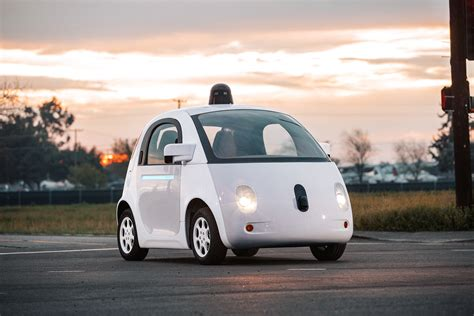
\includegraphics[width=5cm]{googlecar}
  \caption{Self driving car di Google.}
  \label{fig:google}}
  \qquad
  \begin{minipage}{5cm}
  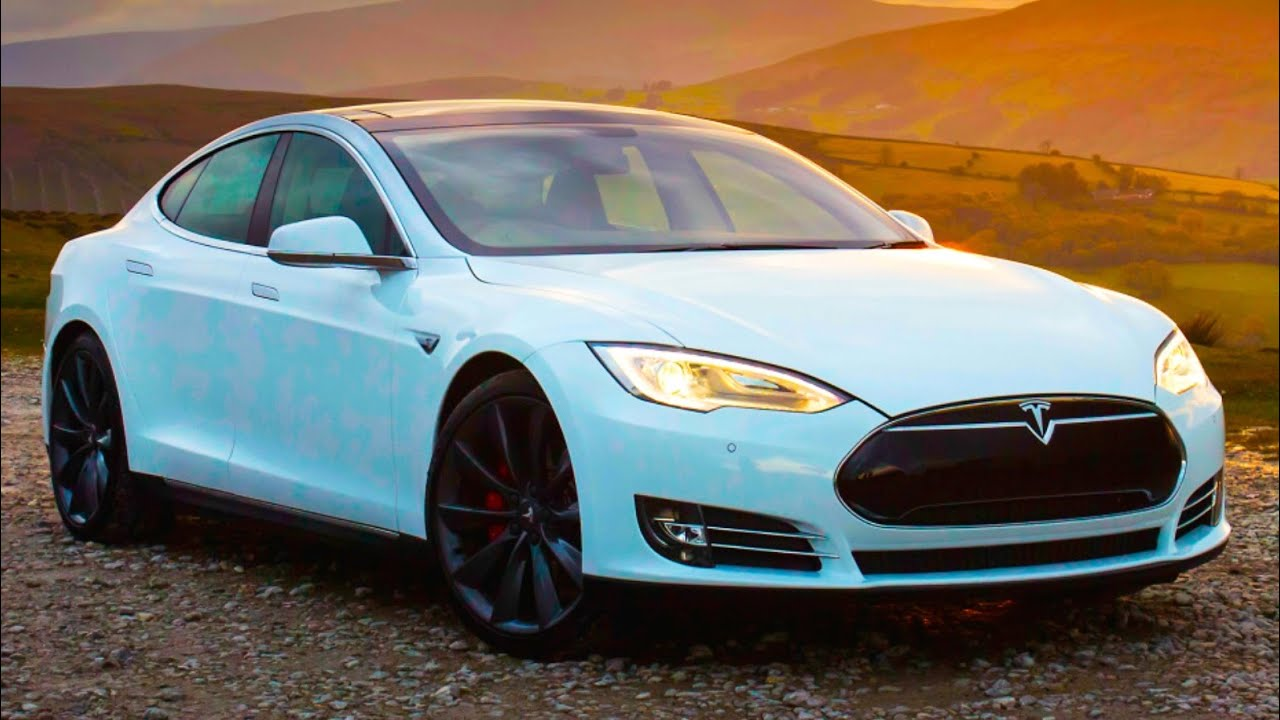
\includegraphics[width=5cm]{tesla}
  \caption{Self driving car di Tesla.}
  \label{fig:tesla}
  \end{minipage}
  \end{figure}
Grandi aziende quali \emph{Google} e \emph{Tesla} hanno già sviluppato
dei propri modelli  (Figura \ref{fig:google} e Figura\ref{fig:tesla}) e l'interesse in questo campo è sempre in  maggior crescita. Per poter funzionare correttamente, i veicoli a guida autonoma sfruttano il Machine Learning e le \emph{reti neurali}. Una macchina acquisisce immagini
dall'ambiente circostante attraverso varie camere e sensori. Queste immagini vengono passate a una rete neurale che, in base alle informazioni raccolte, decide l'azione da compiere (sterzare, accelerare, frenare ecc\dots).
L'utilizzo del Machine Learning ha permesso un notevole avanzamento nello sviluppo di questo settore ma  esistono ancora molte problematiche relative a sicurezza ed affidabilità.\\

Una vulnerabilità molto importante sono i cosiddetti \emph{Adversarial attacks}. Il meccanismo di questi attacchi è molto semplice:
gli input della rete  subiscono una modifica volontaria, impercettibile a occhio umano ma in grado di causare errori di  classificazione.  Questi errori possono portare, ad esempio, una macchina ad accelerare quando
dovrebbe frenare. È fondamentale quindi studiare tali attacchi per verificare la robustezza dei modelli di apprendimento.
In questa Tesi abbiamo studiato, iniettato e verificato l'efficacia di  alcuni degli attacchi forniti dalla libreria python \emph{Adversarial Robustness Toolbox}. Gli attacchi scelti sono stati iniettato all'interno
di LearningByCheating, un modello di guida autonoma preaddestrato che gira sul simulatore di guida urbana Carla.
Il lavoro è così suddiviso:
\begin{itemize}
  \item \textbf{Capitolo 1:} Fondamenti teorici alla base dei sistemi intelligenti;
  \item \textbf{Capitolo 2:} Fondamenti di guida autonoma;
  \item \textbf{Capitolo 3:} Dependability e security;
  \item \textbf{Capitolo 4:} Strumenti utilizzati: vengono presentati \emph{l'Adversarial Robustness Toolbox} e il simulatore \emph{Carla};
  \item \textbf{Capitolo 5:} Il lavoro svolto: attacchi scelti e motivazioni, iniezione e risultati;
  \item \textbf{Capitolo 6:} Conclusioni e possibili sviluppi futuri.
  
\end{itemize}



\chapter{Sistemi Intelligenti}

\section{Intelligenza Artificiale}

\begin{figure}
    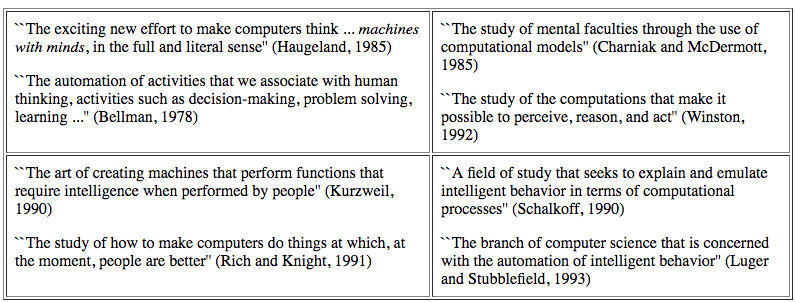
\includegraphics[width=\linewidth]{aidef}
    \caption{Possibili definizioni di Intelligenza artificiale \cite{aima}.}
    \label{fig:ai}
  \end{figure}
Dare un'unica definizione di intelligenza artificiale risulta estremamente difficile a causa della vastità
e dell'interdisciplinarietà dell'argomento. Soltanto nella Figura \ref{fig:ai} ne troviamo addirittura otto, tutte valide, ma forse
la descrizione  migliore per i nostri scopi  è quella data dal padre di questa disciplina, John Mccarthy:
'' L'Intelligenza Artificiale è la scienza volta alla creazione di macchine  \emph{intelligenti},
più nello specifico di \emph{programmi intelligenti}.'' \cite{ai}.
\subsection{Agenti e ambienti}
Il concetto di macchina intelligente può essere ulteriormente
astratto dall'idea di \textbf{agente computazionale intelligente}. Esaminiamo adesso questa definizione.
Un \textbf{agente} è un'entità che compie azioni
e percepisce informazioni da un ambiente.

\begin{figure}
  \centering
  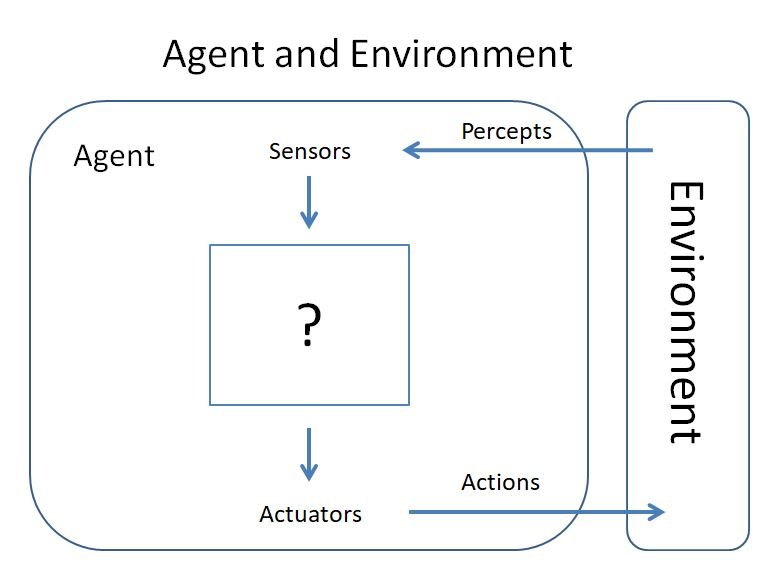
\includegraphics[scale=0.4]{agent}
  \caption{Agente computazionale \cite{aima}.}
  \label{fig:agente}
\end{figure}

Un agente si comporta in modo \textbf{intelligente} quando:
\begin{itemize}
  \item le sue azioni sono appropriate alle circostanze e ai suoi scopi,
  \item è flessibile per ambienti e scopi dinamici,
  \item impara dall'esperienza,
  \item fa le scelte \textbf{giuste} date le sue limitazioni percettive e computazionali. Un agente tipicamente
  non può osservare l'ambiente direttamente; ha una memoria e un tempo per agire molto limitati.
\end{itemize}
 Un agente \textbf{computazionale} è un agente le cui decisioni possono essere descritte in termini di una
 computazione. Questo significa che una decisione può essere scomposta in una serie di operazioni primitive,
 implementabili in un dispositivo fisico \cite{PooleMackworth17}.
 \subsection{Intelligenza e performance}
 Abbiamo detto che un agente è intelligente quando compie le \emph{scelte giuste}. Ma cosa significa fare la scelta giusta?
 Rispondiamo a questa domanda in un modo molto banale: considerando le \emph{conseguenze} del comportamento di un agente.
 Un agente si muove all'interno di un ambiente e compie una sequenza di azioni in base alle informazioni che riceve.
 Queste azioni causano una variazione allo stato dell'ambiente. Se la variazione è desiderabile, l'agente ha fatto le scelte giuste.
 La nozione di desiderabilità è catturata da una \textbf{misura di prestazione (performance measure)} che valuta una qualunque sequenza di azioni.
 Ovviamente non esiste una performance measure globale; solitamente viene costruita appositamente  per uno specifico problema.
 Le specifiche dell'agente, dell'ambiente e della misura di prestazioni vengono raggruppate nell'\textbf{ambiente di lavoro (task environment)},
 attraverso la descrizione PEAS (Performance,Environment,Actuators,Sensors) \cite{aima}.
 \begin{figure}
  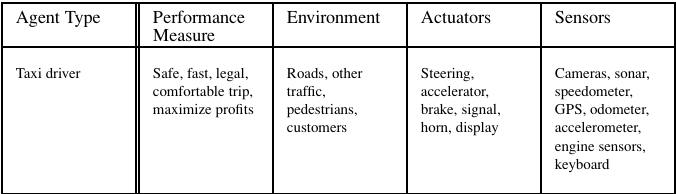
\includegraphics[width=\linewidth]{peas_taxi.png}
  \caption{Descrizione PEAS dell'ambiente di lavoro di un taxi automatico \cite{aima}.}
  \label{fig:taxi}
 \end{figure}
 La Figura \ref{fig:taxi} riassume un esempio di descrizione PEAS dell'ambiente di lavoro di un taxi.
\subsection{Razionalità}
Ciò che abbiamo descritto fin'ora ci permette di verificare in modo quantitativo l'intelligenza di un agente.
Espandiamo questa idea introducendo la nozione di \textbf{razionalità}.
Cosa sia razionale in qualsiasi momento dipende da quattro elementi:
\begin{itemize}
  \item la misura di prestazioni;
  \item la conoscenza a priori dell'agente;
  \item le azioni che l'agente può compiere;
  \item la sequenza di percezioni fino a quel momento.
\end{itemize}
Questo ci porta alla definizione di \textbf{Agente Razionale}:
      \begin{center}
      \emph{per ciascuna sequenza di percezioni, un agente razionale seleziona un'azione che massimizza il valore atteso della performance measure, data l'evidenza 
      fornita dalla sequenza di percezioni e dalla conoscenza a priori dell'agente}
      \end{center}
La razionalità non significa \textbf{onniscienza}. Un agente deve essere in grado di prendere decisioni anche quando
non ha a disposizione tutte le informazioni necessarie a compiere l'azione perfetta. Un agente razionale massimizza \emph{il valore atteso} della performance
basandosi sulla sua conoscenza pregressa dell'ambiente, ma  non sempre un ambiente è completamente osservabile. Per questo motivo sono
fondamentali la fase di raccolta delle informazioni (\textbf{information gathering}) e di apprendimento (\textbf{learning}). Per poter
migliorare le prestazioni, un  agente deve essere in grado di raccogliere la massima quantità possibile di informazioni
e di aggiungere tali informazioni alla propria base di conoscenza. Questo permette una scelta sempre migliore delle azioni da compiere \cite{aima}.
\subsection{Scopo dell'IA}
Lo scopo scientifico  dell'IA è quello di studiare i principi e i meccanismi che rendono il comportamento intelligente possibile, sia
nei sistemi naturali che in quelli artificiali. Lo scopo ingegneristico di questa disciplina è la costruzione di dispositivi fisici
in grado di comportarsi in modo intelligente. Da queste basi si sono sviluppati un innumerevole quantità di branche, tra cui le più importanti sono \cite{ai}:
\begin{itemize}
  \item \textbf{logical AI},
  \item \textbf{search},
  \item \textbf{knowledge and reasoning},
  \item \textbf{planning},
  \item \textbf{learning from experience},
  \item \textbf{genetic programming}.
\end{itemize}
\begin{figure}
  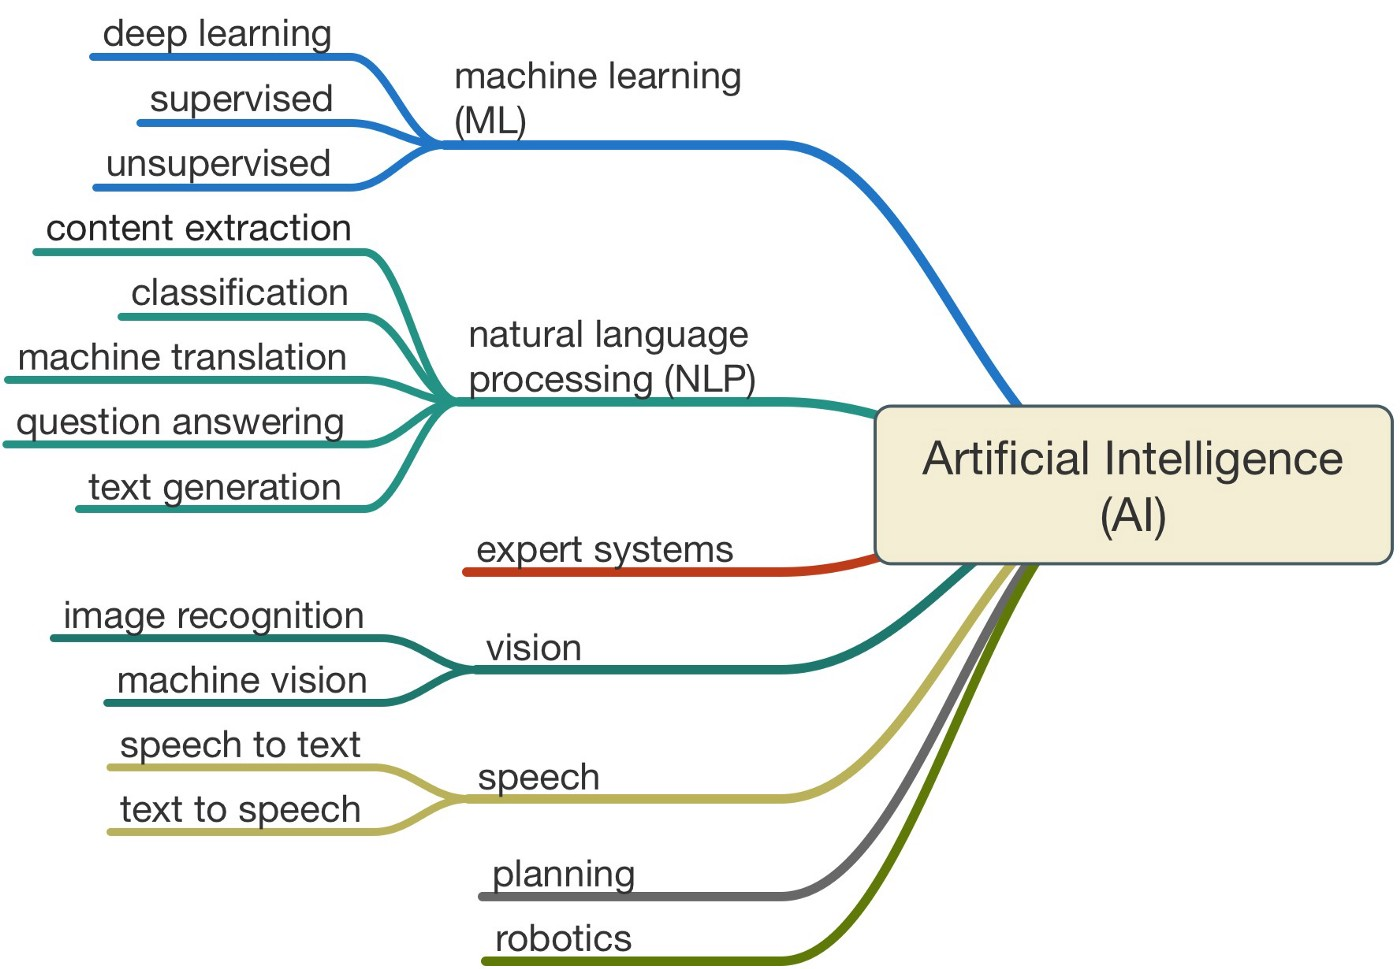
\includegraphics[width=\linewidth]{aibranches}
  \caption{Applicazioni dell'IA \cite{branch}.}
  \label{fig:branches}
\end{figure}
In Figura \ref{fig:branches} vengono riportate alcune delle applicazioni di maggior successo dei \emph{Sistemi Intelligenti}.
Il settore delle Self driving Car si basa in particolare su \textbf{Machine Learning} applicato alla \textbf{Computer Vision}.

\section{Machine Learning}
Il \textbf{Machine Learning (ML)} è una branca dell'intelligenza artificiale dedicata allo studio e allo sviluppo
di algoritmi che migliorano le prestazioni attraverso l'esperienza \cite{mlwiki}. L'abilità di un algoritmo di migliorare dall'esperienza
automaticamente è fondamentale, perchè è impossibile scrivere programmi  che sappiano a priori tutte le possibili situazioni in cui 
un agente potrebbe ritrovarsi. Inoltre l'ambiente in cui l'agente è inserito può mutare nel tempo \cite{aima}. Consideriamo il caso dei mercati finanziari.
Un programma creato per prevedere i prezzi delle azioni di domani deve essere in grado  di adattarsi alle variazioni improvvise causate, ad esempio,
da una crisi globale.
\subsection{Problemi di apprendimento ben definiti}
Iniziamo ad approfondire i concetti di apprendimento automatico considerando alcuni task di apprendimento. Più precisamente:
\begin{defn}\label{def:learn}
  Si dice che un programma \textbf{impara} dall'esperienza E rispetto, a una classe di tasks T e una misura di prestazioni P,
  se la sua prestazione nei tasks in T, misurata da P, migliora con l'esperienza E.
\end{defn}
Dalla definizione \ref{def:learn} possiamo specificare diversi problemi di apprendimento, ad esempio \cite{Mitchell97}:
\begin{itemize}
  \item \textbf{Task T}: giocare a scacchi;
  \item \textbf{Misura di prestazioni P}: percentuale di partite vinte contro gli avversari;
  \item \textbf{Esperienza E}: giocare partite di prova contro se stesso.
\end{itemize}


Ogni problema di learning consiste nel prendere la conoscenza a priori e i dati ricevuti (l'esperienza E) e 
trasformarli in una rappresentazione  interna utilizzata da un agente per prendere decisioni. La rappresentazione
può corrispondere con i dati stessi ricevuti ma di solito è una sintesi compatta e significativa. 
In definitiva, per specificare una determinata tecnica di apprendimento è quindi necessario affrontare le seguenti\cite{PooleMackworth17} questioni:
\begin{itemize}
  \item \textbf{Task} Un task di apprendimento è una qualsiasi attività che può essere appresa da un agente;
  \item \textbf{Feedback} Durante l'apprendimento a un agente viene fornito un riscontro in base alla correttezza delle azioni svolte. Il riscontro può essere un premio o una punizione.  In base ad esso un agente modifica le proprie azioni
  migliorando così la propria esecuzione su un determinato task;
  \item \textbf{Rappresentazione} Come detto in precedenza, l'esperienza deve influenzare la rappresentazione interna di un agente.
  Gran parte del Machine Learning è focalizzato nel contesto di una specifica rappresentazione (es. reti neurali);
  \item \textbf{Online e Offline} Nel learning offline, tutti i training examples sono disponibili prima dell'azione di un agente. Nel learning online,
  gli esempi vengono ricevuti durante l'esecuzione;
  \item \textbf{Misura di Successo} Per sapere se un agente ha effettivamente imparato, è necessaria una misura di successo. La misura NON riguarda le prestazioni sui dati di addestramento, bensì le prestazioni su nuove esperienze;
  \item \textbf{Bias} Con il termine \emph{bias} si intende la tendenza a preferire un'ipotesi rispetto a un'altra, concetto fondamentale nel processo di scelta;
  \item \textbf{Noise} Una delle proprietà più importanti per un algoritmo di apprendimento è la capacità di gestione di dati condizionati.
  Infatti, nella pratica, i dati possono spesso risultare imperfetti o in alcuni casi incompleti;
  \item \textbf{Interpolazione e Estrapolazione} L'interpolazione riguarda le previsioni tra i  casi per i quali si possiedono dei dati (ad esempio approssimare una funzione dati alcuni valori di essa), l'estrapolazione comporta invece 
  previsioni che vanno oltre i dati conosciuti.
\end{itemize}
\subsection{Forme di Learning}
Gli algoritmi di Machine Learning sono suddivisi in diverse classi, a seconda del risultato desiderato.
\begin{figure}
  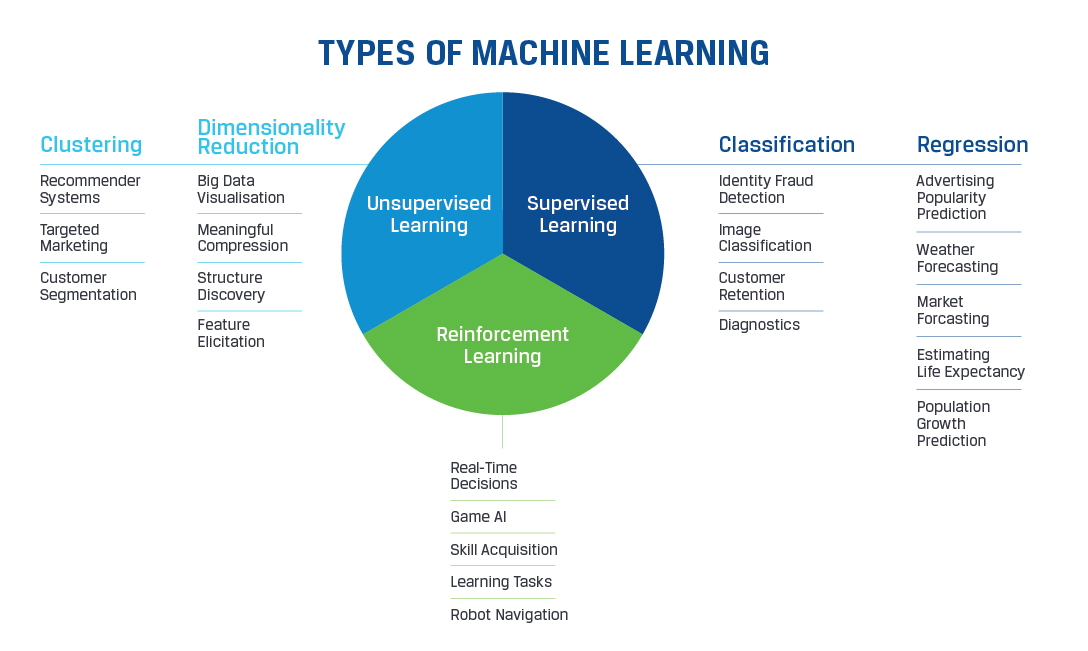
\includegraphics[width=\linewidth]{learning.jpg}
  \caption{Tre maggiori tipi di learning \cite{learn}.}
  \label{fig:ml}
\end{figure}
In Figura \ref{fig:ml} vengono mostrate le tre maggiori classi.
\subsubsection{Deep Supervised Learning}
La forma più comune di Machine Learning è il supervised learning. Consideriamo il caso in cui si voglia addestrare un classificatore
che sappia riconoscere i diversi tipi di segnali stradali. Si colleziona un dataset composto da immagini di segnali stradali, ciascuno di esso con la rispettiva categoria (stop, limite di velocità,
divieto di sosta ecc.). Queste immagini compongono il \textbf{training set}. Durante l'apprendimento, vengono mostrate alla macchina  le immagini del training set. Per ciascuna immagine l'algoritmo produce un output della forma di un vettore di punteggi, uno per ogni categoria.
Si calcola una funzione che misura l'errore (\textbf{loss function}) fra l'output prodotto e l'output desiderato. In base all'errore commesso l'algoritmo modifica dei paramentri interni, detti pesi, 
in modo da ridurlo. Per aggiustare il vettore dei pesi in modo corretto , l'algoritmo di apprendimento utilizza una tecnica detta \emph{Gradient Descent}. Ad ogni errore commesso, il vettore dei pesi viene aggiustato nella direzione di massima decrescita dell'errore, fino a raggiungere un minimo locale. La fase di addestramento termina quando si raggiunge il minimo errore possibile, calcolato come la media della funzione di errore su ogni immagine del dataset.
Terminato il training, la prestazione del classificatore viene misurata su un differente dataset di immagini, detto \textbf{test set}. Questo serve a verificare
la capacità di generalizzazione della macchina, andando a controllare la correttezza degli output su input sconosciuti.

\begin{figure}
  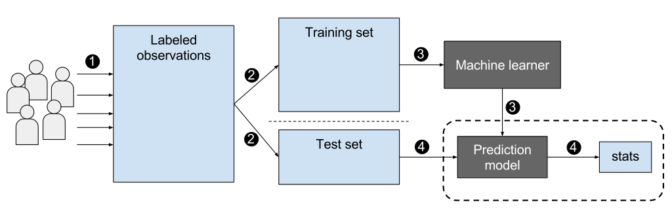
\includegraphics[width=\linewidth]{sup.png}
  \caption{Supervised Learning \cite{sup}.}
  \label{fig:sup}
\end{figure}

Una buona fetta delle applicazioni pratiche utilizza classificatori lineari su caratteristiche modellate a mano. 
Un classificatore binario calcola una somma pesata delle componenti del cosidetto \textbf{feature vector}. Se la somma è sopra una certa soglia, 
l'input è classificato in una certa classe. I classificatori lineari suddividono lo spazio degli input in semplici sottoregioni dette iperpiani, ma contesti come il riconoscimento di immagini o il riconoscimento vocale hanno
bisogno di modelli più complessi, capaci di rilevare  minuscole variazioni su caratteristiche importanti (\textbf{selettività}) e di ignorare anche grandi variazioni su caratteristiche irrilevanti al contesto, come ad esempio una rotazione dell'immagine (\textbf{invarianza}). La scelta delle caratteristiche rilevanti è quindi una
fase fondamentale del processo di learning. Tradizionalmente, la scelta delle features veniva costruita direttamente dagli sviluppatori, il che comportava una grande richiesta di abilità ingegneristica e di competenza nel dominio di lavoro.
Grazie al Deep  Learning  il processo di estrazioni di features rilevanti viene automatizzato con una procedura di apprendimento a scopo generale.
Un'architettura di deep learning è formata da uno stack multilivello di moduli elementari, tutti (o la maggior parte) sottoposti a learning, e la maggior parte dei quali
calcola una mappatura non lineare tra input-output. Ciascun livello aumenta sia la selettività che l'invarianza della rappresentazione. 
Maggiore è la profondità dello stack, maggiore è la complessità della funzione di scelta, capace di rilevare i più piccoli cambiamenti a dettagli rilevanti \cite{deep}.

\subsubsection{Deep FeedForward Neural Networks}

Le reti neurali feedforward sono uno dei modelli computazionali di maggior successo nell'ambito del deep learning. Lo sviluppo in questo campo è stato influenzato  dallo
studio sulla struttura del cervello umano e sulle modalità di trasmissioni di informazioni tra neuroni. L'obiettivo di una rete feedforward  è l'approssimazione di una funzione $f*$ che, nel caso di un classificatore mappa
un vettore di feature \textbf{x} a una categoria \textbf{y}. Una rete feedforward definisce una funzione $y=f(x;\theta)$ e apprende il valore di $\theta$ che permette
la miglior approssimazione possibile. Questo tipo di reti viene detto \textbf{feedforward} perchè i dati passano dall'input x, alle computazioni che definiscono f, e infine all'output y. Non vi sono cicli 
nei quali risultati di calcoli interni sono reinseriti all'interno della rete. Quando le reti includono anche cicli vengono dette \textbf{reti ricorrenti}.
Uno schema di una rete feedforward  è presentato in Figura \ref{fig:ann}. I livelli intermedi sono detti \textbf{hidden (nascosti)} perchè nel \textbf{training set} non vengono esplicitati
gli output desiderati  per ciascuno di questi livelli. Ogni livello nascosto rappresenta una funzione e la funzione totale è data dalla composizione di queste funzioni. Per esempio,
se abbiamo 3 livelli la funzione completa sarà $f(x) = f^{3}(f^{2}(f^{1}(x)))$. Il singolo livello è composto da molte \textbf{unità} che agiscono in parallelo, ciascuna rappresentante una funzione da vettore a scalare \cite{bengio}.
\begin{figure}
  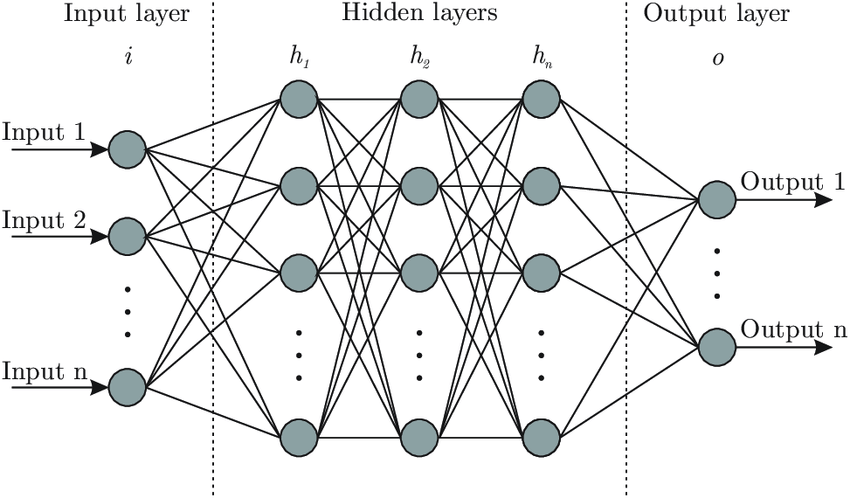
\includegraphics[scale=0.3]{ann.png}
  \caption{Schema base di una rete neurale \cite{ann}.}
  \label{fig:ann}
\end{figure}

La generica i-esima unità  riceve un vettore di input dalle unità del livello precedente, indicati con $X_j$. $X_j$ viene trasmesso all'unità opportunamente moltiplicato da un peso $W_{ij}$.
Gli input ricevuti dall'i-esima unità costituiscono lo stato di attivazione, rappresentato dalla sommatoria \[\sum_jW_{ij}X_j\] L'output prodotto dall'unità viene calcolato attraverso la funzione $f$, detta funzione di attivazione. Il compito della funzione di attivazione è quello di controllare
se lo stato di attivazione supera una certa soglia. Quando questo avviene l'unità trasmette alle unità del livello successivo \cite{mazzetti}.
\begin{figure}
  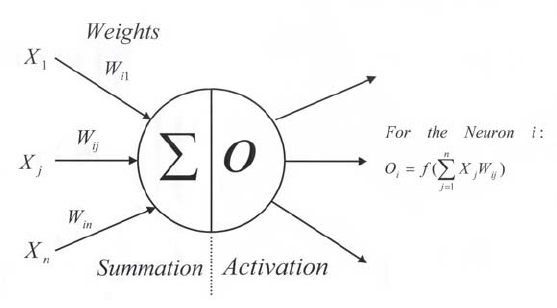
\includegraphics[scale=0.5]{nnunit.png}
  \caption{Un "neurone" artificiale \cite{unit}.}
  \label{fig::unit}
\end{figure}
\begin{figure}
  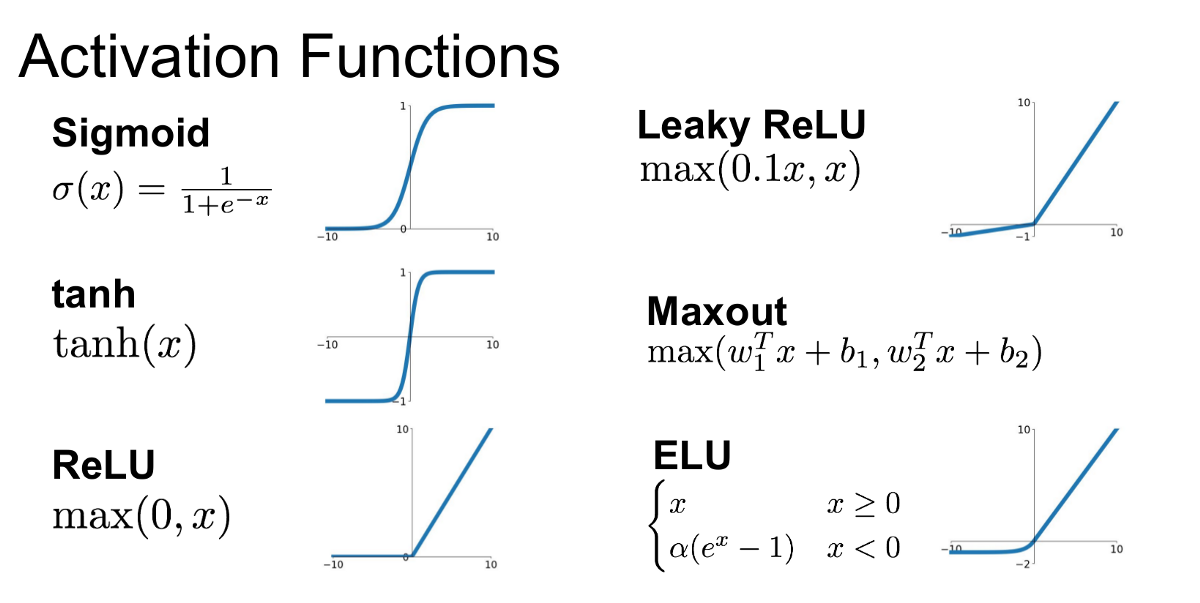
\includegraphics[scale=0.2]{actfun.png}
  \caption{Alcune funzioni di attivazione \cite{act}.}
  \label{fig:act}
\end{figure}

\subsubsection{Learning nei neural network}
Il learning di una rete neurale avviene solitamente (nel caso dell'object recognition) in modalità supervisionata.  Si vuole determinare un vettore dei pesi $\vec{w}$ che permetta alla rete di produrre l'output corretto per ciasun esempio nel training set.
L'idea di base è quella di usare il gradient descent, ma in una rete multilivello il problema è ulteriormente complicato dalla presenza degli \textbf{hidden layers}. Mentre nell'output layer l'errore che si commette in ciascuna fase di addestramento è esplicito, l'errore presente nei livelli nascosti
non è immediato da calcolare, in quanto nel training set non sono presenti i valori che i nodi nascosti devono assumere. Il problema viene risolto trasmettendo a ritroso
l'errore commesso dall'output layer ai livelli nascosti, con un algoritmo detto di \textbf{back-propagation}.
\begin{figure}[h]
  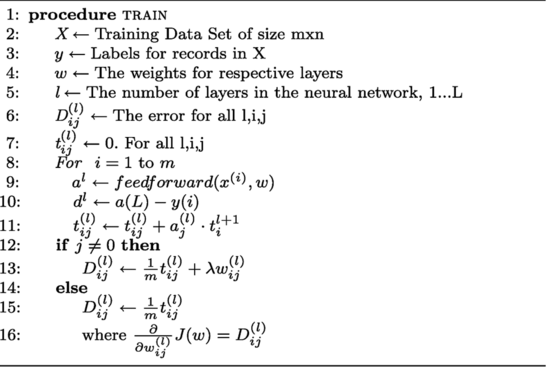
\includegraphics[scale=0.5]{back.png}
  \caption{Pseudocodice della back-propagation \cite{back}.}
  \label{fig:back}
\end{figure}
\subsubsection{Reti Convoluzionali}
Nel contesto dell'object-detection le reti più utilizzate sono le reti convoluzionali. Le reti convoluzionali sono  progettate per processare dati in forma 
matriciale, come immagini e audio. La loro architettura è strutturata in una serie di fasi. Le prime fasi sono composte da due tipi di layer: \textbf{convolutional layers}
e \textbf{pooling layers.}
Le unità in un layer convoluzionale sono organizzate in feature maps, addette a riconoscere alcune caratteristiche di un input. Ciascuna unità è collegata
a un sottoinsieme di unità delle feature maps nei precedenti livelli attraverso un gruppo di pesi detto \textbf{filter bank} e utilizza una funzione di attivazione non lineare come una ReLU. Tutte le unità di una feature map condividono 
la stessa filter bank, e diverse feature maps usano diverse filter bank. L'aggregazione di unità in feature maps è motivata dalla struttura dell'input. Nei dati in forma matriciale, gruppi di valori locali sono spesso fortemente correlati,
formando pattern locali che vengono facilmente riconosciuti. La condivisione di pesi tra unità  diverse è spiegata notando come un pattern possa apparire in qualsiasi parte dell'immagine, e l'utilizzo di una filter bank garantisce invarianza alla località.
Passando ai pooling layer essi hanno il compito di "fondere" features semanticamente simili,tipicamente calcolando il massimo tra un gruppo di unità di una feature map. Questo causa una riduzione nelle dimensioni dell'input che viene poi passato
ai layer successivi, La riduzione delle dimensione è fondamentale per garantire efficienza computazionale e per aumentare l'invarianza alle piccole perturbazioni.
Due o più fasi di convoluzione e pooling sono seguite da altri layer convoluzionali e completamente connessi. Le filter banks vengono addestrate con algoritmi di backpropagation \cite{deep}.
\begin{figure}[h]
  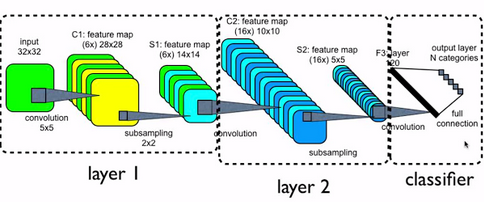
\includegraphics[width=\linewidth]{conv.png}
  \caption{Rete neurale convoluzionale \cite{cnn}.}
  \label{fig:conv}
\end{figure} 

\subsection{Adversarial Examples}
\begin{figure}[h]
  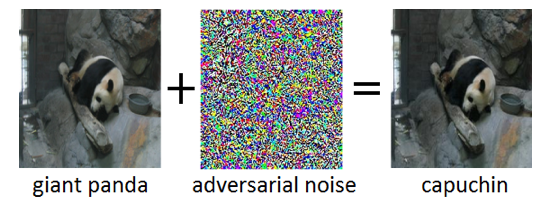
\includegraphics[width=\linewidth]{AdversarialExample_Panda.png}
  \caption{Adversarial example \cite{art2018}.}
  \label{fig:adv}
\end{figure}

Nonostante gli ottimi risultati raggiunti, le reti neurali sono state dimostrate essere vulnerabili ai cosiddetti \emph{adversarial examples} \cite{art2018}. Gli adversarial
examples sono input intenzionalmente modificati che risultano essere molto simili agli input originali per gli esseri umani, ma che causano decisioni scorrette
da parte della rete. La vulnerabilità delle reti a questo tipo di attacchi rappresenta un grande rischio di sicurezza nelle applicazioni pratiche come i veicoli a guida autonoma. Studiarli
è quindi necessario per identificare le limitazioni degli algoritmi di learning attuali, dando così spunti per migliorare la robustezza dei modelli.



    
\myChapter{Fondamenti di guida autonoma}
Lo sviluppo tecnologico nel campo dell'intelligenza artificiale ha permesso una grande evoluzione nel campo della guida autonoma. L'interesse per questo 
settore è guidato dai seguenti vantaggi che questi veicoli possono potenzialmente portare\cite{advantages}:
\begin{itemize}
    \item \textbf{Riduzione degli incidenti} Una grossa parte degli incidenti stradali(fino al $90\%$ )sono dovuti a errori umani. Eliminarli
    significherebbe ridurre notevolmente il numero di infortuni e salvare delle vite.
    \item \textbf{Riduzione del traffico} Grazie al controllo automatico si possono evitare le situazioni di congestione che avvengono naturalmente sulle strade.
    Oltre a migliorare il deflusso veicolare, questo porterebbe anche  una riduzione delle emissioni di CO2 e del consumo di benzina, causate dalle macchine ferme nel traffico.
    \item \textbf{Migliore capacità stradale} L'ottimizzazione del trafico potrebbe portare un notevole incremento nella capacità autostradale. La capacità
    di monitorare in modo costante l'ambiente circostante e reagire istantaneamente renderebbe più sicuro viaggiare a velocità maggiori e con meno spazio tra ciascun veicolo.
    \item \textbf{Accessibilità} Attualmente  molte persone anziane  e/o con disabilità sono escluse dal viaggio in automobile in solitaria. Le self-driving car rappresentano un'opportunità
    di indipendenza per queste categorie, che potrebbero così muoversi senza dover ricorrere a soluzioni esterne.
\end{itemize}
\begin{figure}
    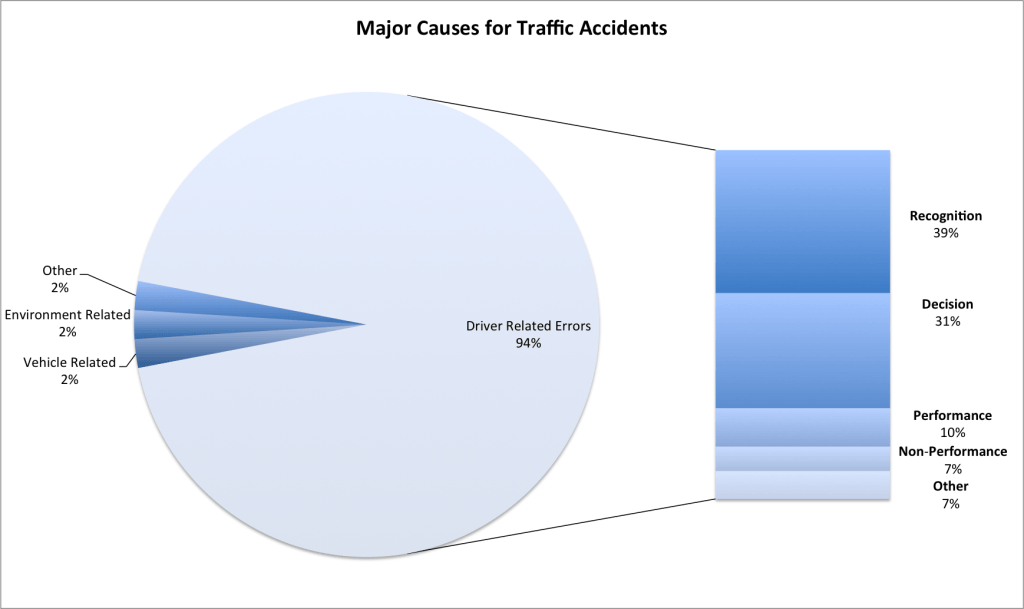
\includegraphics[width=\linewidth]{accidents.png}
    \caption{Maggiori cause di incidenti stradali ad Austin tra il 2005 e il 2007\cite{accid}}
    \label{fig:accid}
\end{figure}
Attualmente però non si puo parlare ancora di guida completamente autonoma, ma di sistemi di guida assistita. Restano ancora molte problematiche aperte, soprattutto 
da un punto di vista legale\cite{legal} etico\cite{Lin2015}. Per questo, e per i problemi di emph{dependability} che verrano illustrati nei prossimi paragrafi, lo sviluppo
di veicoli autonomi è in molti casi ancora in fase prototipale. La ricerca è quindi fondamentale per portare a miglioramenti significativi.
\section{Livelli di automazione}
Nel 2014 la \textbf{SAE international} ha pubblicato lo standard J3016, col quale vengono definiti sei liveli di autonomia, in base a quanto un guidatore deve intervenire.
\begin{figure}
    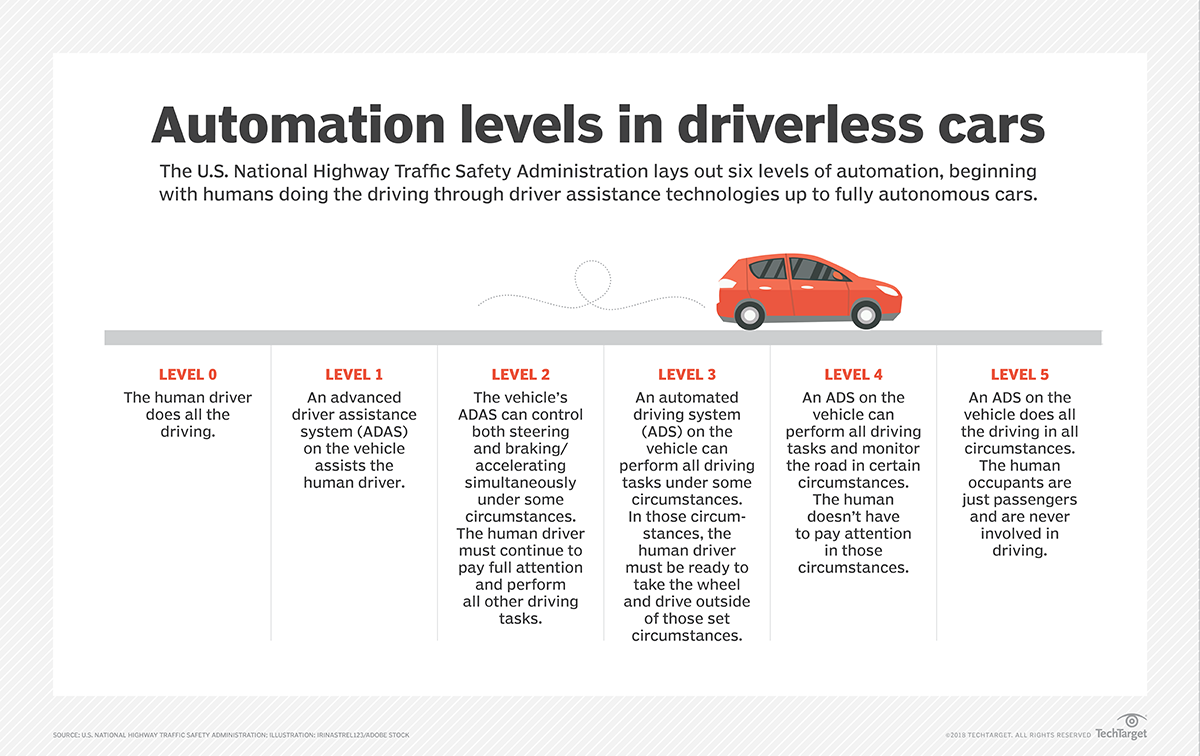
\includegraphics[width=\linewidth]{car_automation_levels.png}
    \caption{livelli di automazione\cite{car}}
    \label{fig:adaslevel}
\end{figure}
\subsubsection{Livello 0}
Nessun tipo di automazione. Il controllo è completamente affidato al conducente.
\subsubsection{Livello 1: Assistenza alla guida}
Il conducente si occupa di tutti gli aspetti della guida. Viene supportato da sistemi elettronici che possono  segnalare la presenza di pericoli attraverso segnali visivi e acustici.
Vengono classificati di livello 1 anche i veicoli con una singola funzione di assistenza automatizzata(ad esempio il controllo automatico della velocità).
\subsubsection{Livello 2: Automazione Parziale}
Il conducente deve mantenere il controllo del veicolo in ogni istante ma le le varie funzioni vengono automatizzate da 
due o più sistemi avanzati di assistenza alla guida(\textbf{sistemi ADAS}). Questi sistemi includono:
\begin{itemize}
    \item Adaptive Cruise Control- controllo automatico della velocità
    \item Lane-Keeping Assist - controllo dello sterzo per impedire l'uscita dalla corsia
    \item Automatic Emergency Braking -  controllo del freno per le situazioni di emergenza
\end{itemize}
\subsubsection{Livello 3: Automazione condizionale}
La guida è completamente automatizzata ma non in tutti i momenti del viaggio. Il conducente viene avvisato quando deve riprendere il controllo ed è tenuto a rispondere
in modo appropriato. Se questo non avviene, il sistema arresta il veicolo nel modo più sicuro possibile.
\subsubsection{Livello 4: Alta Automazione}
Il viaggio è completamente gestito dal sistema. Il conducente non è tenuto a intervenire in nessun momento. La completa autonomia è garantita però a patto che non esistano limitazioni come ad esempio condizioni
metereologiche fortemente avverse.
\subsubsection{Livello 5: Automazione totale}
Sistema completamente autonomo. Non vi è alcuna limitazione ed è tutto gestito dal sistema interno in qualunque momento. 
\subsection{La situazione attuale}
Al momento in commercio esistono veicoli fino al secondo livello(Tesla AutoPilot, Cadillac Super Cruise, Volvo Pilot Assist ecc.). I veicoli di livello 3 e 4 sono ancora in fase prototipale
ma aziende come Honda e Audi promettono  di avere modelli in commercio già dal 2021\cite{honda}. Il livello 5 sembra ancora lontano, ma il ritmo di sviluppo attuale fa ben sperare per i prossimi anni.
    
\section{Visione Artificiale}
La visione dell'ambiente circostante è la questione focale nello sviluppo di un veicolo a guida autonoma. Per poter "vedere", una macchina utilizza diversi sensori:
\begin{itemize}
    \item  Camere,
    \item Radar,
    \item Lidar.
\end{itemize}
\begin{figure}[h]
    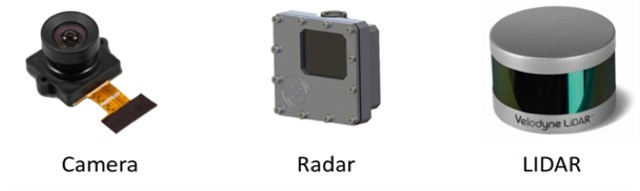
\includegraphics[width = \linewidth]{sensori.jpg}
    \caption{I sensori più utilizzati \cite{lid}.}
    \label{fig:lid}
\end{figure}
\subsection{Camere}
Le videocamere utilizzate sono profondamente diverse dalle normali videocamere in vendita. Sono progettate in modo da avere un campo visivo molto ampio,
minore risoluzione (migliori performance) e per resistere ad alte  e basse temperature. Restano però limitate in situazioni di bassa visibilità.     
\subsection{Radar}
Il compito dei radar è principalmente quello di rilevare ostacoli e situazioni di pericolo imminente. In base alle informazioni raccolte l'auto accelera o frena. 
I radar si rilevano utili anche nella fase di parcheggio.
\subsection{Lidar}
I lidar sono dispositivi il cui funzionamento è simile a quello dei radar. La differenza principale sta nel segnale utilizzato: i radar usano onde radio mentre i lidar usano impulsi luminosi.
I lidar sono particolarmente utili per la rilevazione di pedoni e per riconoscere i segnali stradali.
\begin{figure}[h!]
    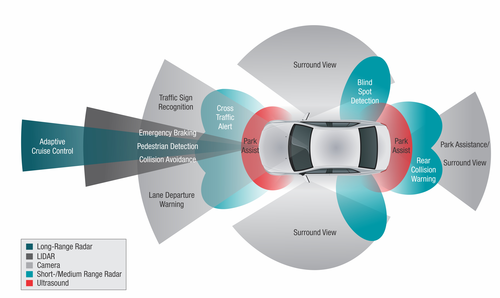
\includegraphics[scale=0.6]{01-autonomous-car-sensors_TI.png}
    \caption{Sensori in una macchina autonoma \cite{sensors}.}
    \label{fig:sensors}
\end{figure}
\newpage
\subsection{Dai sensori agli attuatori}

Tutti i sensori sono fondamentali perchè ciascuno di esso compensa i punti deboli dell'altro. Una videocamera non funziona bene in condizioni di nebbia intensa, ma un radar sì. Un radar però non riconosce se
un semaforo è verde o rosso, mentre una camera sì. Nella Figura \ref{fig:sensors} sono mostrate le funzioni svolte da ciascun sensore.


Le informazioni raccolte dai sensori vengono passate al "livello" sottostante, nel quale il sistema interno sceglie la prossima azione da compiere.
Il modello decisionale più utilizzato è una rete neurale convoluzionale. Il deep learning si è dimostrato estremamente potente in quest'ambito, fornendo
ottimi risultati per l'object recognition. L'azione scelta viene passata agli attuatori (freno, sterzo, acceleratore) che provvedono ad eseguirla.
\begin{figure}[h]
    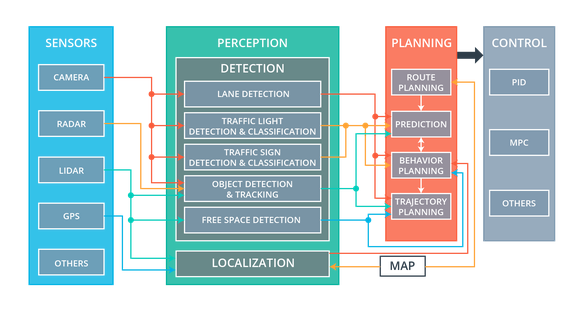
\includegraphics[width=\linewidth]{plan.png}
    \caption{Il processo decisionale \cite{giacaglia}.}
    \label{fig:giacaglia}
\end{figure}
\myChapter{Dependability e Security}
I veicoli a guida autonoma appartengono alla categoria dei sistemi critici. Un sistema critico è un sistema il cui malfunzionamento può provocare danni
considerati inacettabili. Questi includono danni a oggetti di valore, danni ambientali e nei casi piu gravi, il ferimento o addirittura la morte delle persone.
Per garantire che un tale sistema operi nel modo più sicuro possibile è necessario analizzare tutti i fattori che possono portare a  un fallimento irreversibile.

La \textbf{dependability} è la capacità di un sistema di fornire un servizio sul quale fare affidamento in modo giustificato \cite{tax}.
Essa viene suddivisa in 3 categorie:
\begin{itemize}
    \item Attributi,
    \item Minacce,
    \item Mezzi di Raggiungimento.
\end{itemize}
\begin{figure}[h]
    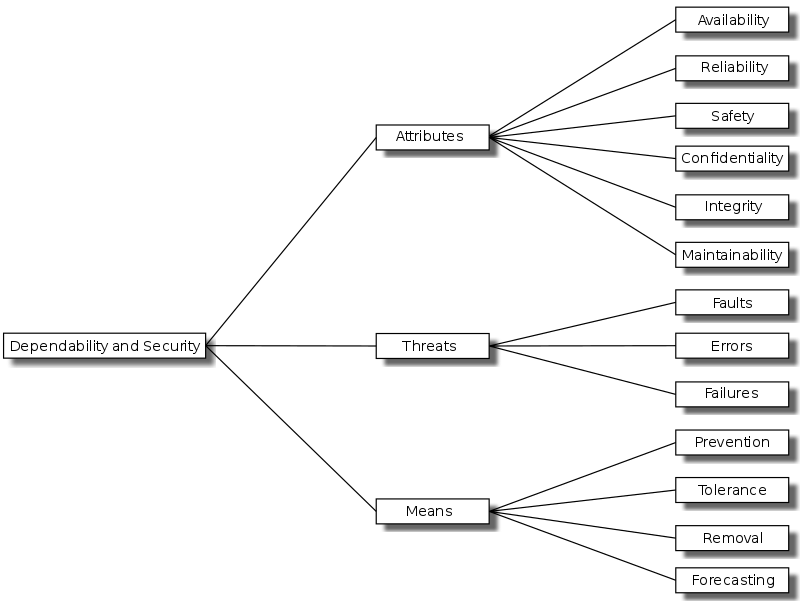
\includegraphics[width = \linewidth]{dep.png}
    \caption{Tassonomia  della dependability \cite{dep}.}
    \label{fig:dep}
\end{figure}
\section{Attributi}
La dependability comprende i seguenti attributi:
\begin{itemize}
    \item \textbf{availability}: disponibilità del servizio corretto;
    \item \textbf{reliability}: stabilità del servizio corretto;
    \item \textbf{safety}: assenza di conseguenze catastrofiche sull'utente e sull'ambiente;
    \item \textbf{integrity}: assenza di alterazioni improprie al sistema;
    \item \textbf{maintainability}: capacità di subire modifiche e riparazioni.
\end{itemize}
Quando si considera la \textbf{security} è necessario specificare un ulteriore attributo: la confidentiality, ovvero la mancata divulgazione di informazioni non 
autorizzata. La security è composta da confidentiality, integrity e availability.
\section{Mezzi di raggiungimento}
Nel corso degli anni si sono sviluppate molte metodologie per raggiungere dependability e security. Tali metodologie possono essere raggruppate in quattro macrocategorie:
\begin{itemize}
    \item \textbf{fault prevention}: mezzi per prevenire l'occorrenza e l'introduzione di guasti;
    \item \textbf{fault tolerance}: mezzi per evitare fallimenti di servizio quando sono presenti dei guasti;
    \item \textbf{fault removal}: mezzi per ridurre numero e gravità dei guasti;
    \item \textbf{fault forecasting}: mezzi per stimare numero, incidenza futura e probabili conseguenze di guasti.
\end{itemize}
Fault prevention e fault tolerance portano al conseguimento della dependability mentre fault removal e fault forecasting sono i mezzi di validazione.
\section{Minacce}
Le maggiori minacce per la dependability sono i \textbf{guasti} (faults in inglese). I guasti hanno varie cause e portano agli \textbf{errori}. Un errore può causarne altri fino a propagarsi
al di fuori dei confini del sistema. Quando ciò avviene, si verifica un \textbf{fallimento}. Un fallimento è la situazione in cui il servizio fornito
è diverso dal servizio corretto.
\begin{figure}[h]
    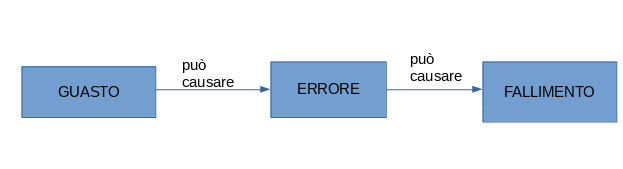
\includegraphics[width=\linewidth]{chain.png}
    \caption{Catena guasto-errore-fallimento.}
\end{figure}
\subsection{Tipi di guasti}
I guasti vengono classificati secondo 8 parametri, i quali creano le classi di guasto elementari, mostrate in Figura \ref{fig:tax}.
\begin{figure}[h]
    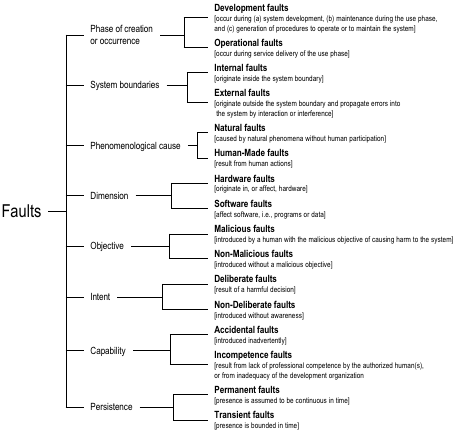
\includegraphics[width = \linewidth]{faults.png}
    \caption{Tassonomia dei guasti \cite{tax}.}
    \label{fig:tax}
\end{figure}
 I diversi tipi di guasto sono raggruppati in tre categorie:
 \begin{itemize}
     \item \textbf{Development faults}: i guasti che avvengono in fase di sviluppo;
     \item \textbf{Physical faults}: i guasti che riguardano l'hardware;
     \item \textbf{Interaction faults}: tutti i guasti causati dall'interazione con l'ambiente esterno.
 \end{itemize}
 \newpage
 \subsubsection{Guasti causati dall'azione umana}
 I guasti sul quale ci concentriamo sono quelli di origine umana . Questi guasti possono essere causati da una mancanza di 
 azioni ove necessarie (omission faults), oppure da azioni che si rilevano essere sbagliate (commision faults). Vengono
 suddivisi in due tipi, sulla base dell'\emph{obiettivo} dello sviluppatore o dell'essere umano che lo causa:
 \begin{itemize}
     \item guasti involontari, causati  accidentalmente senza lo scopo di arrecare danno;
     \item guasti maligni, causati in modo volontario per arrecare danni al sistema durante l'uso.
 \end{itemize}
 I guasti maligni hanno  come scopo la negazione del servizio (denial of service), l'accesso a informazioni confidenziali
 o la modifica impropria di un sistema.
 Vengono raggruppati in due classi:
 \begin{itemize}
     \item \textbf{guasti a livello logico}: comprendono virus, worms, bombe logiche ecc\dots;
     \item \textbf{tentativi di intrusione}, anche usando mezzi fisici.
 \end{itemize}
 In entrambi i casi si sfrutta una vulnerabilità di un sistema per ottenerne il pieno controllo (exploit).
 La vulnerabilità solitamente è a livello software ed è causata dall'azione involontaria degli sviluppatori.


\chapter{L'Adversarial Robustness Toolbox}
L'Adversarial Robustness ToolBox (ART)  è una libreria python che permette  lo  sviluppo di difese per i modelli ad apprendimento automatico, rendendoli più sicuri ed affidabili. Questi modelli sono infatti vulnerabili ai cosidetti "esempi antagonisti": dati in input(immagini, testo ecc.) creati specificatamente per produrre una determinata risposta dal modello. L'ART include questi attacchi e fornisce gli strumenti per sviluppare sistemi di difesa contro di essi. In questa sezione ci concentreremo sugli attacchi, descrivendone il funzionamento e una possibile implementazione su modelli ADAS realizzati all'interno del simulatore Carla.
\\

\noindent Gli attacchi presenti nella libreria sono suddivisi nel seguente modo:
\begin{itemize}
\item Evasion Attacks,dove i dati in input vengono modificati fino ad avere un errore di classificazione

\item Poisoning Attacks. In questo caso l'obiettivo è iniettare  dati  costruiti in modo specifico per compromettere la fase di apprendimento. 
Sono particolarmente efficaci nei casi in cui il riaddestramento è frequente.

\item Extraction Attacks. Nei casi in cui il modello di apprendimento non sia direttamente accessibile, questi tipi di attacchi vengono sviluppati per addestrare un modello sostituto che sia funzionalmente equivalente al modello target.
\end{itemize}

\noindent Nel contesto della guida autonoma, ha senso concentrarsi sugli Evasion Attacks.	 Possiamo infatti assumere che il riaddestramento non avvenga con una tale frequenza da giustificare lo sviluppo intensivo di un attacco poisoning.  Per quanto riguarda gli \textbf{Extraction Attacks} 
, muovendoci in un contesto open source e accademico dove i modelli sono liberamente accessibili, hanno un'utilità limitata per i nostri obiettivi.
Passiamo ora a descrivere alcuni degli esempi presenti nel toolbox.

\section{Trasformazioni Spaziali}
I primi attacchi che consideriamo sono quelli che applicano semplici trasformazioni spaziali alle immagini senza modificare i pixel in modo diretto. Si tratta di attacchi molto interessanti in quanto facilmente implementabili. Si tratta infatti  di ruotare, spostare o sovrapporre più immagini.

\begin{tabular}{|p{3cm}||p{3cm}|p{3cm}|p{3cm}|}

 \hline
 \multicolumn{4}{|c|}{Lista di Attacchi} \\
 \hline
 Nome  & Descrizione attacco & Applicabilità &Implementazione in Carla\\
 \hline
 Adversarial Patch   \cite{patch}
 & L'attacco consiste nell'attaccare su un qualsiasi oggetto  una specifica patch. Questa patch  è creata in modo da  causare errori di classificazione. Può prendere qualsiasi forma  e viene addestrata su un'insieme di immagini, nelle quali verrà applicata con dimensioni e rotazione casuali 
 
 & Un attaccante potrebbe semplicemente stampare la patch e attaccarla ad esempio su un cartello stradale, mandando in confusione i sistemi ADAS. Se si vuole utilizzare l'attacco su delle immagini si può semplicemente porre la patch direttamente sull'immagine.

 & È necessario modificare gli oggetti della simulazione(segnali, veicoli). Nello specifico, dobbiamo intervenire sul motore UE4, responsabile della costruzione di tali oggetti   \\
 \hline
Spatial Transformation Attack \cite{spatial-attack}
 
 & Le immagini che arrivano al classificatore vengono sottoposte a rotazione e traslazione fino a causare un errore di classificazione

& L’attacco potrebbe essere iniettato a livello dei sensori di un sistema ADAS, in modo da modificare direttamente i dati in input causando problemi difficilmente rintracciabili. Questo richiede un tampering della telecamera, per imporre la trasformazione voluta alle immagini.

 & Si utilizzano le API fornite dal simulatore per acquisire le immagini create\\


 \hline
 
\end{tabular}
\section{Perturbazione dell'immagine}
In questo caso l'immagine in input viene sottoposta a una perturbazione, ovvero una modifica di un certo numero di pixel in modo da non essere visibile
 all’occhio umano ma in grado di causare misclassificazione. Questi attacchi risultano essere molto simili tra loro, ma spesso una piccola modifica può causare risultati estremamente diversi. Nello specifico l'adversarial sample $\textbf{x'}$ viene definito come:
 
 \begin{gather*}
 \noindent 	 \textbf{x'} = \textbf{x} + \epsilon_{x}\\
  \{ \textbf{x'} \in \mathbb{R}^{m \times n \times 3} |  \argmax_{j} f(x')\neq \argmax_{i} f(x)\}
 \end{gather*}
 dove $\epsilon_{x} \in \mathbb{R}^{m \times n \times 3}$ è la perturbazione aggiunta all'input \cite{thresh-lowpix}.\\\\

 
 

\noindent\begin{tabular}{|p{3cm}||p{3cm}|p{3cm}|p{3cm}|}
 \hline
 \multicolumn{4}{|c|}{Lista di Attacchi} \\
 \hline
 Nome     & Descrizione attacco & Applicabilità &Implementazione in Carla\\
 \hline
 Threshold Attack \cite{thresh-lowpix}
 
 &  Viene imposta una soglia massima $th$ alla perturbazione. Nello specifico l'attacco ottimizza  il vincolo $ \norm{\epsilon_{x}}_{\infty} 	\leq th$ dove $th$ è uno dei seguenti valori \{1, 3, 5, 10\}
   
 
 & Dobbiamo poter perturbare le immagini e successivamente passarle al classificatore.  Per questo l'attacco verrà implementato a livello dell'unità di elaborazione.
 
 &Si utilizzano le python API fornite dal simulatore per avere accesso alla struttura interna dei veicoli, dove risiede il classificatore\\

 
 \hline
 
 Low Pixel Attack \cite{thresh-lowpix}
 &
 È una variazione del threshold attack usando la norma 0 al posto della norma infinito.
 
 & Poichè l'attacco è concettualmente identico al threshold attack anch'esso verra iniettato nell'unità di elaborazione
 
 &Si accede alla struttura interna dei veicoli con le python API\\
 \hline
 Decision Tree Attack \cite{decTree}
 
 &  Si sfrutta la struttura ad albero del classificatore,  cercando  un cammino dalla foglia originale ad una  foglia che corrisponde a una classe diversa.   Infine si applica la perturbazione all'esempio

& L'attacco viene iniettato all'interno dell'unità di elaborazione del sistema di guida autonoma.

& Si accede alla struttura interna dei veicoli con le python API \\
  \hline
\end{tabular}


\bibliographystyle{plain}
\bibliography{bibliografia}




%--------------------------------------------------------------
\end{document}
%--------------------------------------------------------------
